\documentclass{beamer}

\usepackage{babel}
\usepackage{tikz}
%\usetheme{boxes}
\usepackage[utf8]{inputenc}
\usepackage{amsmath}
\usepackage{amsthm}
\usepackage{hyperref}
\usepackage{natbib}
\usepackage{tikz}
\usepackage{xcolor}
\usepackage[absolute,overlay]{textpos}
\bibliographystyle{plainnat}
\usecolortheme{crane}

\definecolor{orange}{RGB}{232, 86, 15}
\definecolor{blue}{RGB}{14, 159, 232}
\definecolor{blueblue}{RGB}{50, 90, 160}
\definecolor{yellow}{RGB}{232, 187, 14} 
\definecolor{red}{RGB}{232, 14, 59}
\newtheorem{deff}{Definición}
%Information to be included in the title page:
\institute[]{}

\setbeamercolor{title}{bg=blueblue, fg=white}
\setbeamercolor{subttile}{bg=blueblue, fg=white}
\setbeamercolor{frametitle}{bg=blueblue, fg=white}
\setbeamercolor{block title}{bg=blue, fg=white}
\setbeamercolor{block title alerted}{bg=red, fg=white}
\setbeamercolor{block title example}{bg=yellow, fg=white}
\setbeamercolor{footline}{bg=gray, fg=white}
\beamertemplatenavigationsymbolsempty

	
\newcommand{\indep}{\perp \!\!\! \perp}

\newcommand\blfootnote[1]{%
  \begingroup
  \renewcommand\thefootnote{}\footnote{#1}%
  \addtocounter{footnote}{-1}%
  \endgroup
}


\newcommand\overalert[2]{
	 \only<#1>{
\begin{textblock*}{\textwidth}(.35\textwidth,0.25\textheight)
    \begin{beamercolorbox}[wd=.5\textwidth,center,sep=0.3cm]{block title alerted}
	    #2
    \end{beamercolorbox}
\end{textblock*}
}
}

\newcommand\overexample[2]{
	 \only<#1>{
\begin{textblock*}{\textwidth}(.35\textwidth,0.25\textheight)
    \begin{beamercolorbox}[wd=.5\textwidth,center,sep=0.3cm]{block title example}
	    #2
    \end{beamercolorbox}
\end{textblock*}
}
}


\newcommand\overeblock[2]{
	 \only<#1>{
\begin{textblock*}{\textwidth}(.35\textwidth,0.25\textheight)
    \begin{beamercolorbox}[wd=.5\textwidth,center,sep=0.3cm]{block title}
	    #2
    \end{beamercolorbox}
\end{textblock*}
}
}

\title{Applications and Examples}
\author{Gherardo Varando}
\date{IPL \\ 16 May 2023}
\usepackage[nolist]{acronym}

\newcommand{\Q}{Q_{10}}
\newcommand{\SWC}{SWC}
\newcommand{\GPP}{GPP}
\newcommand{\VPD}{VPD}
\newcommand{\Rbsyn}{Rbsyn}
\newcommand{\RECOsyn}{RECOsyn}
\newcommand{\SWPOTsmdiff}{SWPOTsmdiff}
\newcommand{\SWPOTsm}{SWPOTsm}
\newcommand{\Rb}{Rb}
\newcommand{\E}{\mathbb{E}}
\begin{document}

\begin{acronym}
\acro{DML}[DML]{double machine learning}
\acro{EC}[EC]{eddy covariance}
\acro{GPP}[GPP]{gross primary production}
\acro{LUE}[LUE]{light-use efficiency}
\acro{NEE}[NEE]{net ecosystem exchange}
\acro{NN}[NN]{neural network}
\acro{OOD}[OOD]{out-of-distribution}
\acro{RECO}[RECO]{ecosystem respiration}
\acro{SW}[SW]{incoming shortwaves}
\acro{VPD}[VPD]{vapor pressure deficit}
\acro{NT}[NT]{nighttime}
\acro{DT}[DT]{daytime}
\acro{SIF}[SIF]{solar-induced chlorophyll fluorescence}
\end{acronym}


\begin{frame}
	\titlepage
\end{frame}

\begin{frame}{Common Driver example}
	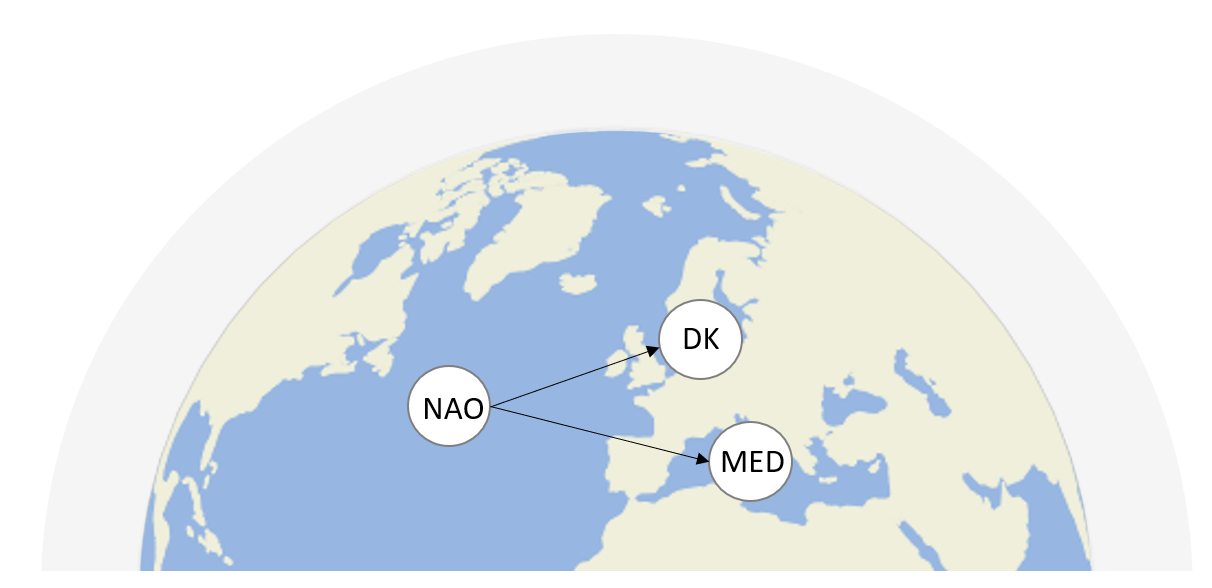
\includegraphics[scale=0.5]{images/ex1}
	\blfootnote{\citet{QuantifyingCausalPathwaysofTeleconnections}}
\end{frame}
\begin{frame}{Double Machine Learning}


	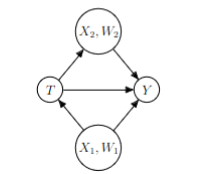
\includegraphics[scale=0.5]{images/dmlgraph}


\begin{align}
    Y = \theta(X)\cdot T + g(X, W).
\end{align}

The parameter $\theta$ describes the direct effect of some variable $T$ on the outcome variable $Y$. 
\begin{align}
Y &= \theta(X)\cdot T + g(X,W)+\epsilon \; &\E[\epsilon|X, W]=0\\
T &= m(X,W) + \eta & \E[\eta|X, W]=0\\
 & & \E[\eta\cdot \epsilon |X,W]=0.
\end{align}
\end{frame}
\begin{frame}
We proceed according to the partialling out method of the double machine learning framework~\cite{Chernozhukov2018}:
\begin{enumerate}
    \item Fit an estimator $\E[Y|X,W]$ of $Y$ on $X$ and $W$,
    \item fit an estimator $\E[T|X,W]$ of $T$ on $X$ and $W$,
    \item compute residuals over $\Tilde{Y} = Y-\E[Y|X,W]$ and $\Tilde{T} = T-\E[T|X,W]$ and
    \item estimate $\hat{\theta} = \arg \min_{\theta \in \Theta} \sum_i (\Tilde{Y} - \theta(X)\cdot \Tilde{T})^2$.
\end{enumerate}
\end{frame}

\begin{frame}{The Q10 model} 
	\begin{align}\label{eq:Q10}
	R_{eco}(X,T)=R_b(X, T)\cdot \Q^{(T-T_{ref})/10}, \end{align} Following
	the example of \cite{Reichstein2022}, we used data from the EC tower in
	Neustift, Austria, from 2003 to 2007 of the FLUXNET2015 dataset and
	generated the data similarly.

	\begin{block}{Synthetic data} 
		\vspace{-0.7cm}
		\small
	\begin{align} \RECOsyn &= \Rbsyn \cdot
		\Q^{0.1\cdot(T-15)},\\ \Rbsyn &= 0.75 \cdot (\tilde{R}^{syn}_b
		- \min(\tilde{R}^{syn}_b) + 0.1\cdot \pi),\label{eq:Rb_zero}\\
	\tilde{R}^{syn}_b &= 0.01 \cdot \SWPOTsm - 0.005 \cdot \SWPOTsmdiff,
	\end{align} 
		\vspace{-0.8cm}
		\begin{itemize}
			\item  $\Rb^{syn}$ describes the base respiration 
			\item The smooth incoming
	potential radiation $\SWPOTsm$ and its smoothed difference quotient
	$\SWPOTsmdiff$ are computed by averaging moving windows of 10 days over
	the incoming potential radiation $SW_{POT}$. 
\item The $\Q$ temperature coefficient is set to $1.5$.
		\end{itemize}
	\end{block}
 
\end{frame}

\begin{frame}{In-situ data}
	Ecosystem respiration is not directly observed at flux towers during
	the day.  It is a latent flux that can only be measured under
	controlled conditions such as a sealed chamber. At night, however, we
	assume $\GPP$ to be zero as there is no photosynthesis occurring, and
	all carbon flow stems from respiration. From all measured data, the
	ones that do not fulfill a certain quality criterion are filtered out
	and gap filled. We will work with measured data only. Only about $10\%$
	of the nighttime data is observed. 
	Thus, we estimate $\Q$ on 4331 data
	points. As predictors we will use the day of the year to account for
	seasonality, vapor pressure deficit $\VPD$, and soil water content
	$\SWC$.  
\end{frame} 

\begin{frame}{Bootstrapped results for synthetic data}
	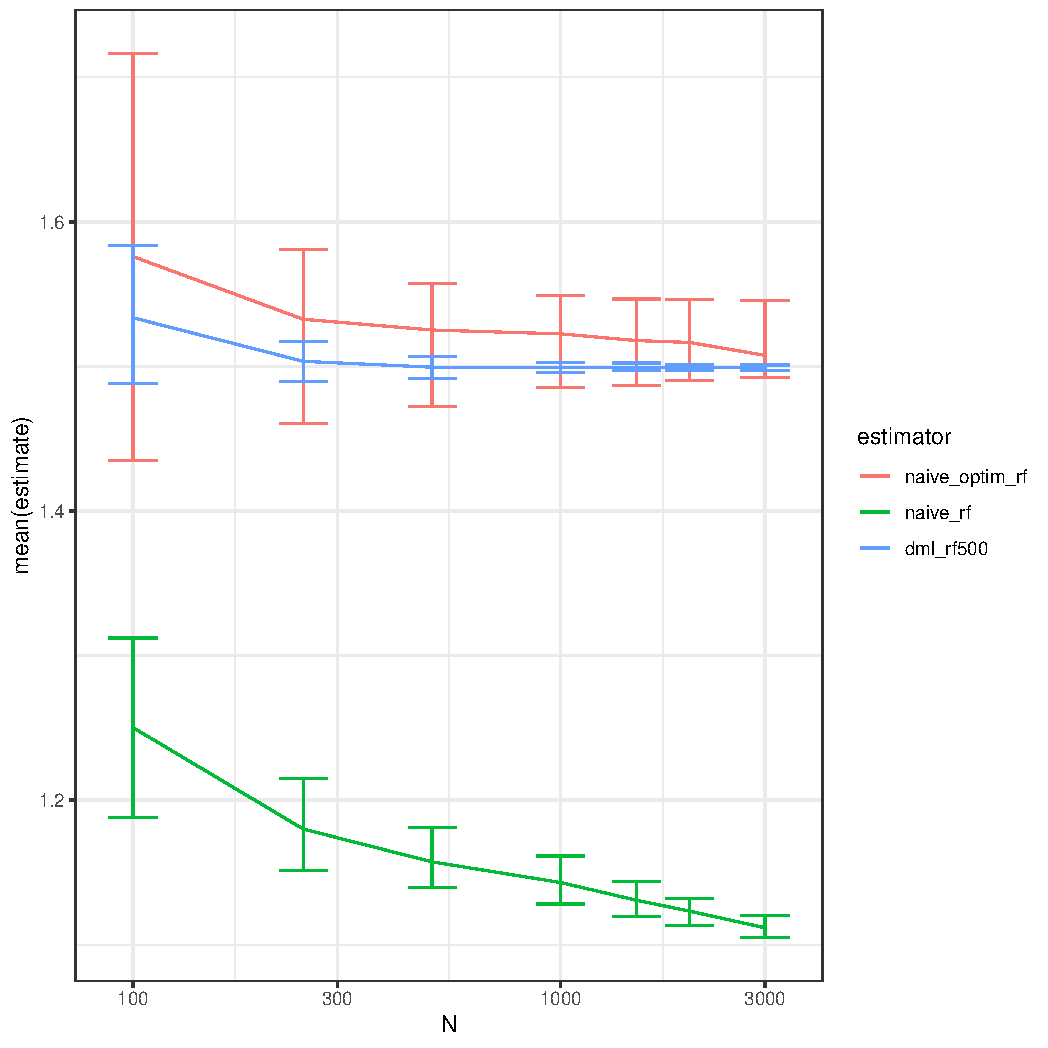
\includegraphics[scale=0.4]{images/avg_estimate_confint_emp}
\end{frame}

\begin{frame}{Bootstrapped results for real data}
	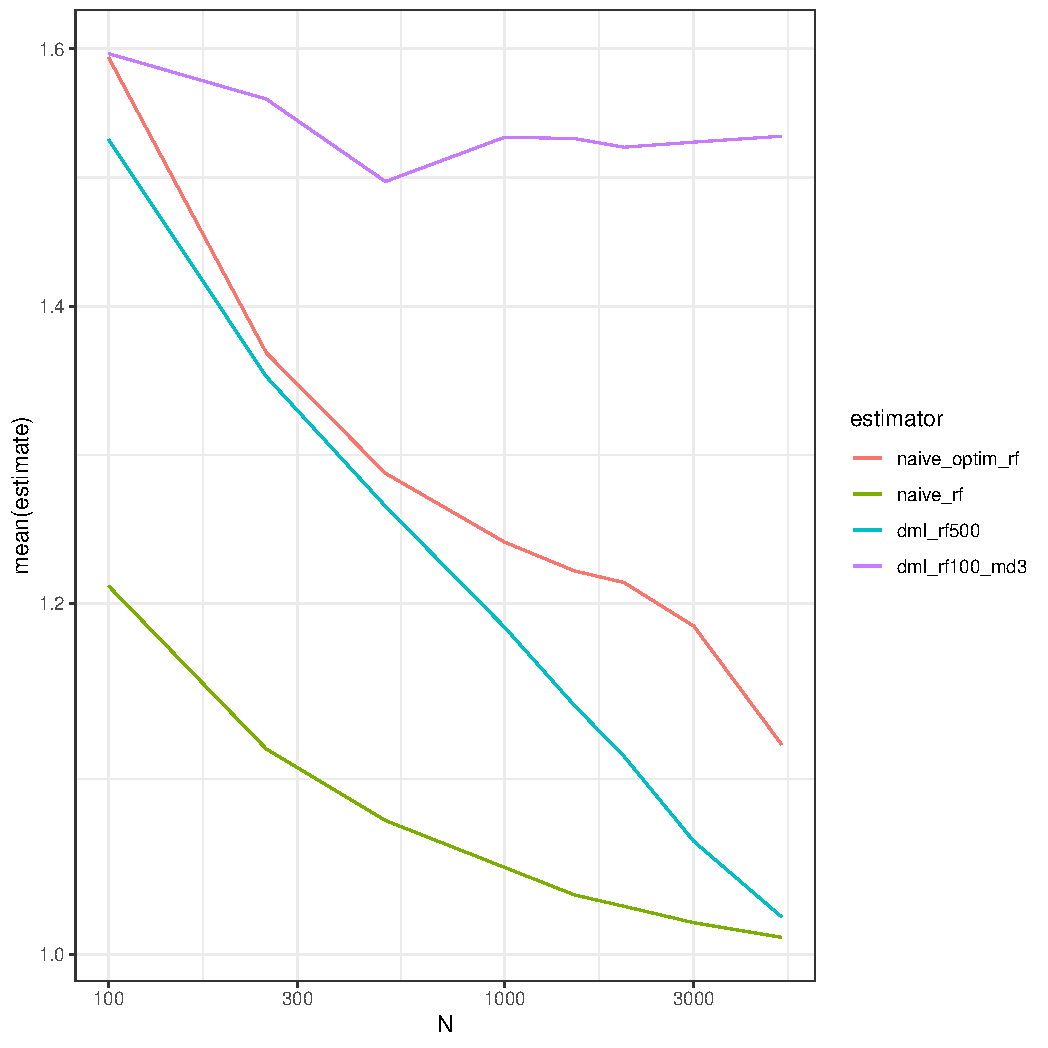
\includegraphics[scale=0.4]{images/avg_estimate}
\end{frame}

\begin{frame}{ENSO Effects on Spring Precipitation in
Australia}
\begin{columns}
    \begin{column}{0.5\textwidth}
        \begin{itemize}
		\item Effect of El Niño Southern Oscillation (ENSO) 
on Australian precipitation (AU) during
spring, and the possible mediation of the 
Indian Ocean Dipole (IOD)~\citep{QuantifyingCausalPathwaysofTeleconnections}
\item monthly NCEP reanalyses covering 1949–2019
\item ENSO (Niño, neutral, Niña), IOD into positive (+), neutral (0) and negative (-) phases; 
	and AU into
above (high) and below (low) average values
 
\end{itemize}
    \end{column}

    \begin{column}{0.45\textwidth}
	    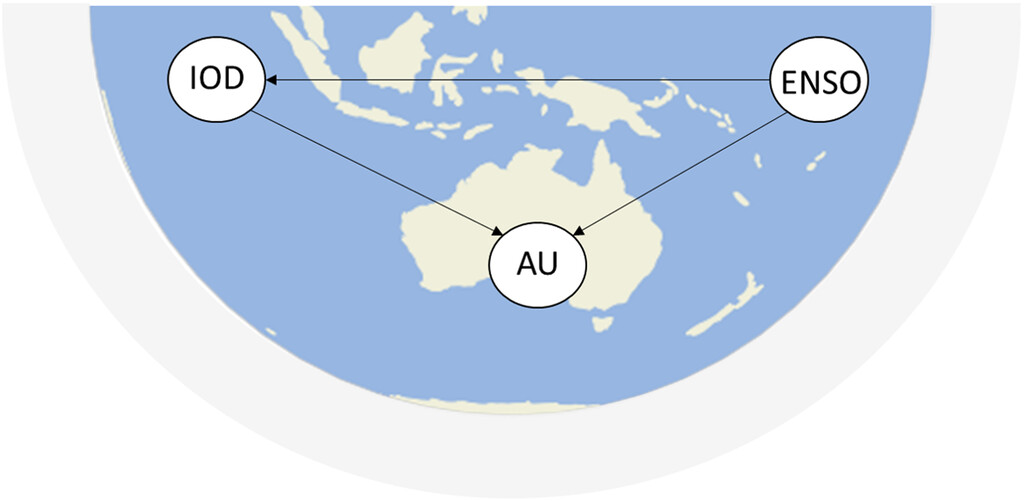
\includegraphics[scale=3]{images/enso-iod-au}
    \end{column}
\end{columns}
  \end{frame}

\begin{frame}[allowframebreaks]
\bibliography{biblio, references1, biblio_causal} 
\end{frame}

\end{document}


